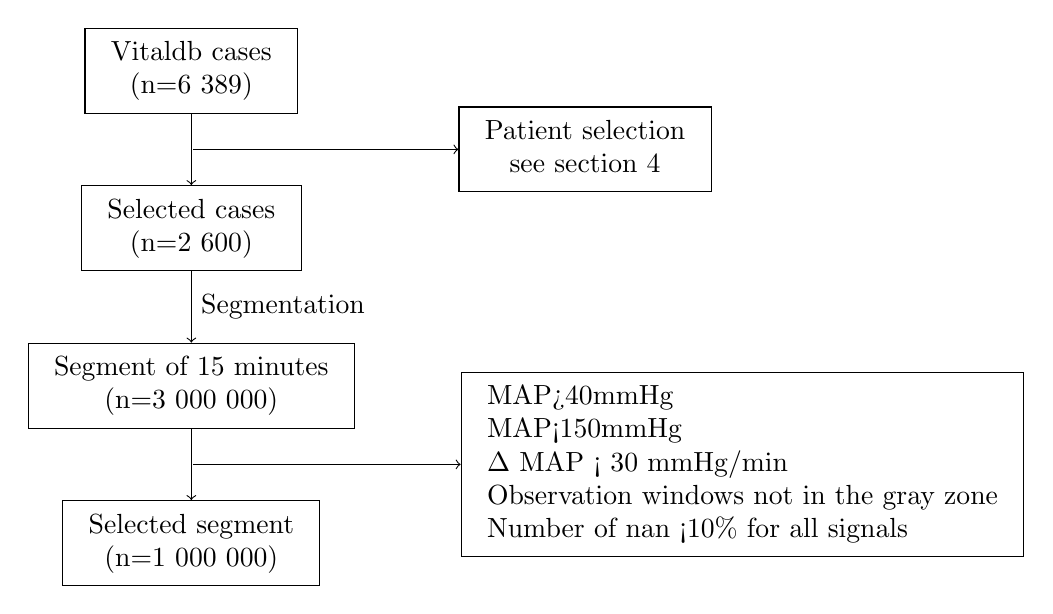
\begin{tikzpicture}
    \node (vdb) at (0, 0) [draw, rectangle, minimum width=2cm, minimum height=1cm] {\begin{tabular}{c} Vitaldb cases \\ (n=6 389) \end{tabular}};

    \node (cases) [draw, rectangle, below of=vdb, yshift= -1cm, minimum width=2cm, minimum height=1cm] {\begin{tabular}{c} Selected cases \\ (n=2 600) \end{tabular}};

    \node (features) [draw, rectangle, below of=cases, yshift= -1cm, minimum width=2cm, minimum height=1cm] {\begin{tabular}{c} Segment of 15 minutes \\ (n=3 000 000) \end{tabular}};

    \node (selected_features) [draw, rectangle, below of=features, yshift= -1cm, minimum width=2cm, minimum height=1cm] {\begin{tabular}{c} Selected segment \\ (n=1 000 000) \end{tabular}};

    \draw [->] (vdb) -- (cases) node (arrow1) [midway, xshift=-1mm] {};
    \draw [->] (cases) -- (features)node [midway, right] {Segmentation};
    \draw [->] (features) -- (selected_features) node (arrow3) [midway, xshift=-1mm] {};


    \node (patient_select) [draw, rectangle, right of=vdb, xshift= 4cm, yshift=-1cm, minimum width=2cm, minimum height=1cm] {\begin{tabular}{c} Patient selection \\ see section 4 \end{tabular}};
    \draw [<-] (patient_select) -- (arrow1);

    \node (feature_select) [draw, rectangle, right of=features, xshift= 6cm, yshift= -1cm, minimum width=2cm, minimum height=1cm] {\begin{tabular}{l} MAP>40mmHg \\ MAP<150mmHg \\ $\Delta$ MAP < 30 mmHg/min \\ Observation windows not in the gray zone \\ Number of nan <10\% for all signals \end{tabular}};
    \draw [<-] (feature_select) -- (arrow3);
\end{tikzpicture}